\documentclass[a4paper]{article}

\usepackage{inputenc}
\usepackage[british,UKenglish]{babel}
\usepackage{amsmath}
%\usepackage{titlesec}
\usepackage{color}
\usepackage{graphicx}
\usepackage{fancyref}
\usepackage{hyperref}
\usepackage{float}
\usepackage{scrextend}
\usepackage{setspace}
\usepackage{xargs}
\usepackage{multicol}
\usepackage{nameref}

\usepackage{sectsty}
\usepackage{multicol}
\usepackage{multirow}
\usepackage[procnames]{listings}
\usepackage{appendix}

\newcommand\tab[1][1cm]{\hspace*{#1}}
\hypersetup{colorlinks=true, linkcolor=black}
\interfootnotelinepenalty=10000

\newcommand{\cleancode}[1]{\begin{addmargin}[3em]{3em}\texttt{\textcolor{cleanOrange}{#1}}\end{addmargin}}
\newcommand{\cleanstyle}[1]{\text{\textcolor{cleanOrange}{\texttt{#1}}}}


\usepackage[colorinlistoftodos,prependcaption,textsize=footnotesize]{todonotes}
\newcommandx{\commred}[2][1=]{\textcolor{Red}
{\todo[linecolor=red,backgroundcolor=red!25,bordercolor=red,#1]{#2}}}
\newcommandx{\commblue}[2][1=]{\textcolor{Blue}
{\todo[linecolor=blue,backgroundcolor=blue!25,bordercolor=blue,#1]{#2}}}
\newcommandx{\commgreen}[2][1=]{\textcolor{OliveGreen}{\todo[linecolor=OliveGreen,backgroundcolor=OliveGreen!25,bordercolor=OliveGreen,#1]{#2}}}
\newcommandx{\commpurp}[2][1=]{\textcolor{Plum}{\todo[linecolor=Plum,backgroundcolor=Plum!25,bordercolor=Plum,#1]{#2}}}

\def\code#1{{\tt #1}}

\def\note#1{\noindent{\bf [Note: #1]}}

\makeatletter
%% The "\@seccntformat" command is an auxiliary command
%% (see pp. 26f. of 'The LaTeX Companion,' 2nd. ed.)
\def\@seccntformat#1{\@ifundefined{#1@cntformat}%
   {\csname the#1\endcsname\quad}  % default
   {\csname #1@cntformat\endcsname}% enable individual control
}
\let\oldappendix\appendix %% save current definition of \appendix
\renewcommand\appendix{%
    \oldappendix
    \newcommand{\section@cntformat}{\appendixname~\thesection\quad}
}
\makeatother


% "define" Scala
\usepackage[T1]{fontenc}  
\usepackage[scaled=0.82]{beramono}  
\usepackage{microtype} 

\sbox0{\small\ttfamily A}
\edef\mybasewidth{\the\wd0 }

\lstdefinelanguage{scala}{
  morekeywords={abstract,case,catch,class,def,%
    do,else,extends,false,final,finally,%
    for,if,implicit,import,match,mixin,%
    new,null,object,override,package,%
    private,protected,requires,return,sealed,%
    super,this,throw,trait,true,try,%
    type,val,var,while,with,yield},
  sensitive=true,
  morecomment=[l]{//},
  morecomment=[n]{/*}{*/},
  morestring=[b]",
  morestring=[b]',
  morestring=[b]"""
}

\usepackage{color}
\definecolor{dkgreen}{rgb}{0,0.6,0}
\definecolor{gray}{rgb}{0.5,0.5,0.5}
\definecolor{mauve}{rgb}{0.58,0,0.82}

% Default settings for code listings
\lstset{frame=tb,
  language=scala,
  aboveskip=3mm,
  belowskip=3mm,
  showstringspaces=false,
  columns=fixed, % basewidth=\mybasewidth,
  basicstyle={\small\ttfamily},
  numbers=none,
  numberstyle=\footnotesize\color{gray},
  % identifierstyle=\color{red},
  keywordstyle=\color{blue},
  commentstyle=\color{dkgreen},
  stringstyle=\color{mauve},
  frame=single,
  breaklines=true,
  breakatwhitespace=true,
  procnamekeys={def, val, var, class, trait, object, extends},
  procnamestyle=\ttfamily\color{red},
  tabsize=2
}

\lstnewenvironment{scala}[1][]
{\lstset{language=scala,#1}}
{}
\lstnewenvironment{cpp}[1][]
{\lstset{language=C++,#1}}
{}
\lstnewenvironment{bash}[1][]
{\lstset{language=bash,#1}}
{}
\lstnewenvironment{verilog}[1][]
{\lstset{language=verilog,#1}}
{}



%代码段设置
\lstset{numbers=left,
basicstyle=\tiny,
numberstyle=\tiny,
keywordstyle=\color{blue!70},
commentstyle=\color{red!50!green!50!blue!50},
frame=single, rulesepcolor=\color{red!20!green!20!blue!20},
escapeinside=``
}

\graphicspath{ {images/} }
\usepackage{ctex}
\usepackage{graphicx}
\usepackage{color,framed}%文本框
\usepackage{listings}
\usepackage{caption}
\usepackage{amssymb}
\usepackage{enumerate}
\usepackage{xcolor}
\usepackage{bm} 
\usepackage{lastpage}%获得总页数
\usepackage{fancyhdr}
\usepackage{tabularx}  
\usepackage{geometry}
\usepackage{minted}
\usepackage{graphics}
\usepackage{subfigure}
\usepackage{float}
\usepackage{pdfpages}
\usepackage{pgfplots}
\pgfplotsset{width=10cm,compat=1.9}
\usepackage{multirow}
\usepackage{footnote}
\usepackage{booktabs}

%-----------------------伪代码------------------
\usepackage{algorithm}  
\usepackage{algorithmicx}  
\usepackage{algpseudocode}  
\floatname{algorithm}{Algorithm}  
\renewcommand{\algorithmicrequire}{\textbf{Input:}}  
\renewcommand{\algorithmicensure}{\textbf{Output:}} 
\usepackage{lipsum}  
\makeatletter
\newenvironment{breakablealgorithm}
  {% \begin{breakablealgorithm}
  \begin{center}
     \refstepcounter{algorithm}% New algorithm
     \hrule height.8pt depth0pt \kern2pt% \@fs@pre for \@fs@ruled
     \renewcommand{\caption}[2][\relax]{% Make a new \caption
      {\raggedright\textbf{\ALG@name~\thealgorithm} ##2\par}%
      \ifx\relax##1\relax % #1 is \relax
         \addcontentsline{loa}{algorithm}{\protect\numberline{\thealgorithm}##2}%
      \else % #1 is not \relax
         \addcontentsline{loa}{algorithm}{\protect\numberline{\thealgorithm}##1}%
      \fi
      \kern2pt\hrule\kern2pt
     }
  }{% \end{breakablealgorithm}
     \kern2pt\hrule\relax% \@fs@post for \@fs@ruled
  \end{center}
  }
\makeatother
%------------------------代码-------------------
\usepackage{xcolor} 
\usepackage{listings} 
\lstset{ 
breaklines,%自动换行
basicstyle=\small,
escapeinside=``,
keywordstyle=\color{ blue!70} \bfseries,
commentstyle=\color{red!50!green!50!blue!50},% 
stringstyle=\ttfamily,% 
extendedchars=false,% 
linewidth=\textwidth,% 
numbers=left,% 
numberstyle=\tiny \color{blue!50},% 
frame=trbl% 
rulesepcolor= \color{ red!20!green!20!blue!20} 
}

%-------------------------页面边距--------------
\geometry{a4paper,left=2.3cm,right=2.3cm,top=2.7cm,bottom=2.7cm}
%-------------------------页眉页脚--------------
\usepackage{fancyhdr}
\pagestyle{fancy}
\lhead{\kaishu \leftmark}
% \chead{}
\rhead{\kaishu 并行程序设计实验报告}%加粗\bfseries 
\lfoot{}
\cfoot{\thepage}
\rfoot{}
\renewcommand{\headrulewidth}{0.1pt}  
\renewcommand{\footrulewidth}{0pt}%去掉横线
\newcommand{\HRule}{\rule{\linewidth}{0.5mm}}%标题横线
\newcommand{\HRulegrossa}{\rule{\linewidth}{1.2mm}}
\setlength{\textfloatsep}{10mm}%设置图片的前后间距
%--------------------文档内容--------------------

\begin{document}
\renewcommand{\contentsname}{目\ 录}
\renewcommand{\appendixname}{附录}
\renewcommand{\appendixpagename}{附录}
\renewcommand{\refname}{参考文献} 
\renewcommand{\figurename}{图}
\renewcommand{\tablename}{表}
\renewcommand{\today}{\number\year 年 \number\month 月 \number\day 日}

%-------------------------封面----------------
\begin{titlepage}
    \begin{center}
    
\includegraphics[width=0.8\textwidth]{NKU.png}\\[1cm]
    \vspace{20mm}
		\textbf{\huge\textbf{\kaishu{计算机学院}}}\\[0.5cm]
		\textbf{\huge{\kaishu{并行程序设计实验报告}}}\\[2.3cm]
		\textbf{\Huge\textbf{\kaishu{作业二:体系结构及性能相关测试}}}

		\vspace{\fill}
    
    % \textbf{\Large \textbf{并行程序设计期末实验报告}}\\[0.8cm]
    % \HRule \\[0.9cm]
    % \HRule \\[2.0cm]
    \centering
    \textsc{\LARGE \kaishu{姓名\ :\ 熊宇轩}}\\[0.5cm]
    \textsc{\LARGE \kaishu{学号\ :\ 2010056}}\\[0.5cm]
    \textsc{\LARGE \kaishu{专业\ :\ 计算机科学与技术}}\\[0.5cm]
    
    \vfill
    {\Large 2022年3月13日}
    \end{center}
\end{titlepage}

\renewcommand {\thefigure}{\thesection{}.\arabic{figure}}%图片按章标号
\renewcommand{\figurename}{图}
\renewcommand{\contentsname}{目录}  
\cfoot{\thepage\ of \pageref{LastPage}}%当前页 of 总页数


% 生成目录
\clearpage
\tableofcontents
\newpage

%--------------------------Title--------------------------------
\section{实验目标}
\begin{enumerate}
  \item 以矩阵每一列与向量的内积为例,通过编写代码实践cache优化算法。
  \item 以求数组累加和为例,通过编写代码实践两路链式相加、循环展开和递归相加等超标量优化算法。
  \item 利用prof和uprof等工具,通过运行计时和事件计数的方法,量化分析普通算法和优化算法之间的性能差异。
\end{enumerate}

\section{核心代码}
代码仓库地址:\href{https://github.com/suhipek/NKU_parallel_programming/tree/main/2_cache_superscalar_profiling}{Github}

\subsection{高精度计时函数}
由于计时的代码比较复杂,写在main函数中显得太为冗杂。因此将计时代码封装为一个函数,将待测试的函数指针作为参数。实验在X86和ARM平台下都是通过Linux系统进行的,故使用了Linux系统的clock\_gettime函数。
\begin{minted}[mathescape,
               linenos,
               numbersep=5pt,
               gobble=2,
               frame=lines,
               framesep=2mm,
               highlightcolor=green!40]{c}
               
    #include <time.h>
    #include <sys/time.h>
    #define REPT 200
    //...
    void test(int (*func)(int*, int), const char* msg, int* arr, int len)
    {
        timespec start, end;
        double time_used = 0;
        cout << "result: " << func(arr,len) << "    ";
        clock_gettime(CLOCK_REALTIME, &start);
        int repeat = REPT*(int)pow(2,(20-(int)(log2(len))));
        for (int i = 0; i < repeat; i++)
            func(arr, len);
        clock_gettime(CLOCK_REALTIME, &end);
        time_used += end.tv_sec - start.tv_sec; // seconds used
        time_used += double(end.tv_nsec - start.tv_nsec) / 1000000000; // nanoseconds used
        cout << msg << ": " << time_used << endl;
    }
\end{minted}

\subsection{矩阵列向量和向量点积函数}
\subsubsection{平凡算法}
\begin{minted}[mathescape,
               linenos,
               numbersep=5pt,
               gobble=2,
               frame=lines,
               framesep=2mm,
               highlightcolor=green!40]{c}

    #define REPT 200
    //...
    int *common_algo(int mat[N][N], int vec[N], int n)
    {
    
        int *sum = new int[n];
        for (int i = 0; i < n; i++)
        {
            sum[i] = 0;
            for (int j = 0; j < n; j++)
                sum[i] += mat[j][i] * vec[j];
        }
        return sum;
    }
\end{minted}

\subsubsection{优化算法}
\begin{minted}[mathescape,
               linenos,
               numbersep=5pt,
               gobble=2,
               frame=lines,
               framesep=2mm,
               highlightcolor=green!40]{c}

    int *optimized_algo(int mat[N][N], int vec[N], int n)
    {
        int *sum = new int[n];
        for (int i = 0; i < n; i++)
            sum[i] = 0;
        for (int i = 0; i < n; i++)
            for (int j = 0; j < n; j++)
                sum[j] += mat[i][j] * vec[i];
        return sum;
    }
\end{minted}

\subsection{累加函数}
\subsubsection{平凡算法}
\begin{minted}[mathescape,
               linenos,
               numbersep=5pt,
               gobble=2,
               frame=lines,
               framesep=2mm,
               highlightcolor=green!40]{c}

    int common_algo(int *arr, int len)
    {
        int total = 0;
        for (int i = 0; i < len; i++)
            total += arr[i];
        return total;
    }
\end{minted}

\subsubsection{N路链式(循环展开)}
一开始在本实验中,笔者试图使用模板的方式来进行循环展开,然而,GCC编译器展开模板时,最高只能展开900层,而这样还不足以凸显出Cache大小和循环展开代码的性能之间的关系。而二路链式其实是最基本的循环展开方式,因此笔者使用Python编写了一个代码变成器,生成了最多8192路链式相加的代码。
\begin{minted}[mathescape,
               linenos,
               numbersep=5pt,
               gobble=2,
               frame=lines,
               framesep=2mm,
               highlightcolor=green!40]{c}

    int unroll_algo_1024(int *arr, int len)
    {
        int total[1024] = {0};
        for (int i = 0; i < len; i += 1024)
        {
            total[0] += arr[i + 0];
            total[1] += arr[i + 1];
            total[2] += arr[i + 2];
            total[3] += arr[i + 3];
            total[4] += arr[i + 4];
            total[5] += arr[i + 5];
            total[6] += arr[i + 6];
            total[7] += arr[i + 7];
            //...
            //这里真的有1024行代码
            //...
        }
        return common_algo(total, 1024);
    }
\end{minted}

\subsubsection{递归算法}
\begin{minted}[mathescape,
               linenos,
               numbersep=5pt,
               gobble=2,
               frame=lines,
               framesep=2mm,
               highlightcolor=green!40]{c}
    int recursive_algo(int *arr, int len)
    {
        for(int m = len; m>1; m/=2)
            for(int i=0; i< m/2; i++)
                arr[i] = arr[i * 2] +arr[i *2 +1];
        return arr[0];
    }
\end{minted}


\section{实验环境}
\subsection{X86平台}
X86平台使用的是一台笔记本电脑,运行Linuxmint 20.3 una系统,内存8GB,内核版本为Linux 5.4.0-100-generic。CPU为AMD的锐龙移动端处理器R5-3500U,具体参数如下:
\begin{minted}[mathescape,
               linenos,
               numbersep=5pt,
               gobble=2,
               frame=lines,
               framesep=2mm,
               highlightcolor=green!40]{bash}
    suhipek@suhipek-BOHK-WAX9X:~$ lscpu
    Architecture:                    x86_64
    CPU op-mode(s):                  32-bit, 64-bit
    Byte Order:                      Little Endian
    Address sizes:                   43 bits physical, 48 bits virtual
    CPU(s):                          8
    On-line CPU(s) list:             0-7
    Thread(s) per core:              2
    Core(s) per socket:              4
    Socket(s):                       1
    NUMA node(s):                    1
    Vendor ID:                       AuthenticAMD
    CPU family:                      23
    Model:                           24
    Model name:                      AMD Ryzen 5 3500U with Radeon Vega Mobile Gfx
    Stepping:                        1
    Frequency boost:                 enabled
    CPU MHz:                         1223.521
    CPU max MHz:                     2100.0000
    CPU min MHz:                     1400.0000
    BogoMIPS:                        4191.85
    Virtualization:                  AMD-V
    L1d cache:                       128 KiB
    L1i cache:                       256 KiB
    L2 cache:                        2 MiB
    L3 cache:                        4 MiB
    NUMA node0 CPU(s):               0-7
\end{minted}
其中显示的L1数据和指令缓存为四个CPU核心缓存数量的总和,每个CPU核心实际的数据缓存大小为32KB。

\subsection{ARM平台}
ARM平台使用课程提供的服务器,运行CantOS,内核版本Linux 4.14.0-115.el7a.0.1.aarch64,CPU为华为的鲲鹏920,具体参数如下:
\begin{minted}[mathescape,
               linenos,
               numbersep=5pt,
               gobble=2,
               frame=lines,
               framesep=2mm,
               highlightcolor=green!40]{bash}
    [s2010056@master screenFetch]$ lscpu
    Architecture:          aarch64
    Byte Order:            Little Endian
    CPU(s):                96
    On-line CPU(s) list:   0-95
    Thread(s) per core:    1
    Core(s) per socket:    48
    座:                 2
    NUMA 节点:         4
    型号:              0
    CPU max MHz:           2600.0000
    CPU min MHz:           200.0000
    BogoMIPS:            200.00
    L1d 缓存:          64K
    L1i 缓存:          64K
    L2 缓存:           512K
    L3 缓存:           49152K
    NUMA 节点0 CPU:    0-23
    NUMA 节点1 CPU:    24-47
    NUMA 节点2 CPU:    48-71
    NUMA 节点3 CPU:    72-95
\end{minted}

\section{实验过程}

\subsection{矩阵列向量和向量点积}

首先,生成测试数据

\begin{minted}[mathescape,
               linenos,
               numbersep=5pt,
               gobble=2,
               frame=lines,
               framesep=2mm,
               highlightcolor=green!40]{bash}
    g++ -O2 ./mar_vec_gen.cpp -o mar_vec_gen
    ./mar_vec_gen
\end{minted}

然后,运行进行时间测量的shell脚本\href{https://github.com/suhipek/NKU_parallel_programming/blob/main/2_cache_superscalar_profiling/mat_test.sh}{mat\_test.sh},这个脚本会通过编译时宏定义(-D选项)多次编译运行并输出结果
\begin{minted}[mathescape,
               linenos,
               numbersep=5pt,
               gobble=2,
               frame=lines,
               framesep=2mm,
               highlightcolor=green!40]{bash}
    
    ./mat_tesh.sh > res.csv
\end{minted}

之后, 通过perf进行事件计数的性能测量
\begin{minted}[mathescape,
               linenos,
               numbersep=5pt,
               gobble=2,
               frame=lines,
               framesep=2mm,
               highlightcolor=green!40]{bash}
               
    g++ -g -DN=1024 ./matrix_product.cpp -o ./matrix_product # N为矩阵行数
    sudo perf record -e \
    L1-dcache-load-misses,L1-dcache-loads,L1-dcache-prefetches,branches, \
    branch-misses,cycles,instructions,idle-cycles-backend,idle-cycles-frontend, \
    L1-icache-load-misses,L1-icache-loads,branch-load-misses,branch-loads \
    -g -o perf_$(date +%m_%d_%H_%M).data ./matrix_product
\end{minted}

对于ARM平台,则通过qsub命令提交这两个脚本:\href{https://github.com/suhipek/NKU_parallel_programming/blob/main/2_cache_superscalar_profiling/mat_timing.sh}{mat\_timing.sh} 
\href{https://github.com/suhipek/NKU_parallel_programming/blob/main/2_cache_superscalar_profiling/mat_perf.sh}{mat\_perf.sh}

\subsection{累加}

该实验的测试数据可使用上文中实验生成的数据。

首先生成代码,\href{https://github.com/suhipek/NKU_parallel_programming/blob/main/2_cache_superscalar_profiling/mar_vec_gen.cpp}{mar\_vec\_gen.cpp}这个程序会根据\href{https://github.com/suhipek/NKU_parallel_programming/blob/main/2_cache_superscalar_profiling/unroll_sum.h}{unroll\_sum.h}的内容生成中\href{https://github.com/suhipek/NKU_parallel_programming/blob/main/2_cache_superscalar_profiling/unroll_sum.cpp}{unroll\_sum.cpp}中展开的函数:
\begin{minted}[mathescape,
               linenos,
               numbersep=5pt,
               gobble=2,
               frame=lines,
               framesep=2mm,
               highlightcolor=green!40]{bash}
    python3 ./unroll_gen.py
\end{minted}

进行时间测量,与上个实验不同,这个实验的时间测量是在程序内完成的,没有使用编译时宏定义
\begin{minted}[mathescape,
               linenos,
               numbersep=5pt,
               gobble=2,
               frame=lines,
               framesep=2mm,
               highlightcolor=green!40]{bash}
    g++  -DN=65536 ./cumulative.cpp ./unroll_sum.cpp -o cumulative
    ./cumulative > sum_timing.csv
\end{minted}

使用perf进行事件计数
\begin{minted}[mathescape,
               linenos,
               numbersep=5pt,
               gobble=2,
               frame=lines,
               framesep=2mm,
               highlightcolor=green!40]{bash}
    g++ -D USE_FIXED_N -DN=1048576 ./cumulative.cpp ./unroll_sum.cpp -o cumulative
    sudo perf record -e \
    L1-dcache-load-misses,L1-dcache-loads,L1-dcache-prefetches,branches, \
    branch-misses,cycles,instructions,idle-cycles-backend,idle-cycles-frontend, \
    L1-icache-load-misses,L1-icache-loads,branch-load-misses,branch-loads \
    -g -o perf_$(date +%m_%d_%H_%M).data ./cumulative
\end{minted}

对于ARM平台,则通过qsub命令提交这两个脚本:\href{https://github.com/suhipek/NKU_parallel_programming/blob/main/2_cache_superscalar_profiling/sum_timing.sh}{sum\_timing.sh} 
\href{https://github.com/suhipek/NKU_parallel_programming/blob/main/2_cache_superscalar_profiling/sum_perf.sh}{sum\_perf.sh}

\newpage
\section{实验结果}
\subsection{运行计时}
矩阵列向量点积实验运行计时的结果如下图所示,其中,矩阵行列数在实验中以16为步进。
\begin{figure}[!htbp]
\centering
\subfigure[ARM平台]{
\begin{minipage}[t]{0.5\linewidth}
\centering
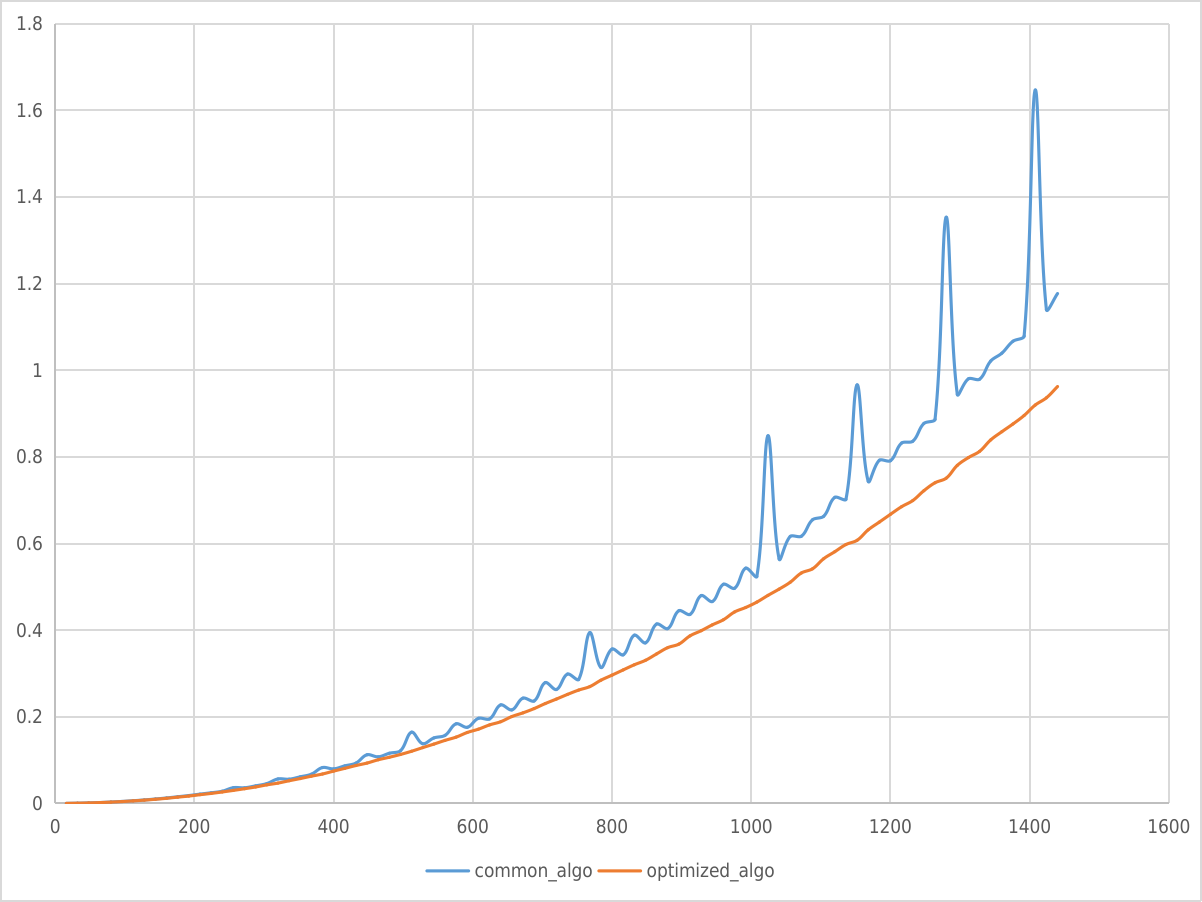
\includegraphics[width=3.2in]{fig/ARM_mat_timing.png}
\label{fig:diff1}
\end{minipage}%
}%
\subfigure[X86平台]{
\begin{minipage}[t]{0.5\linewidth}
\centering
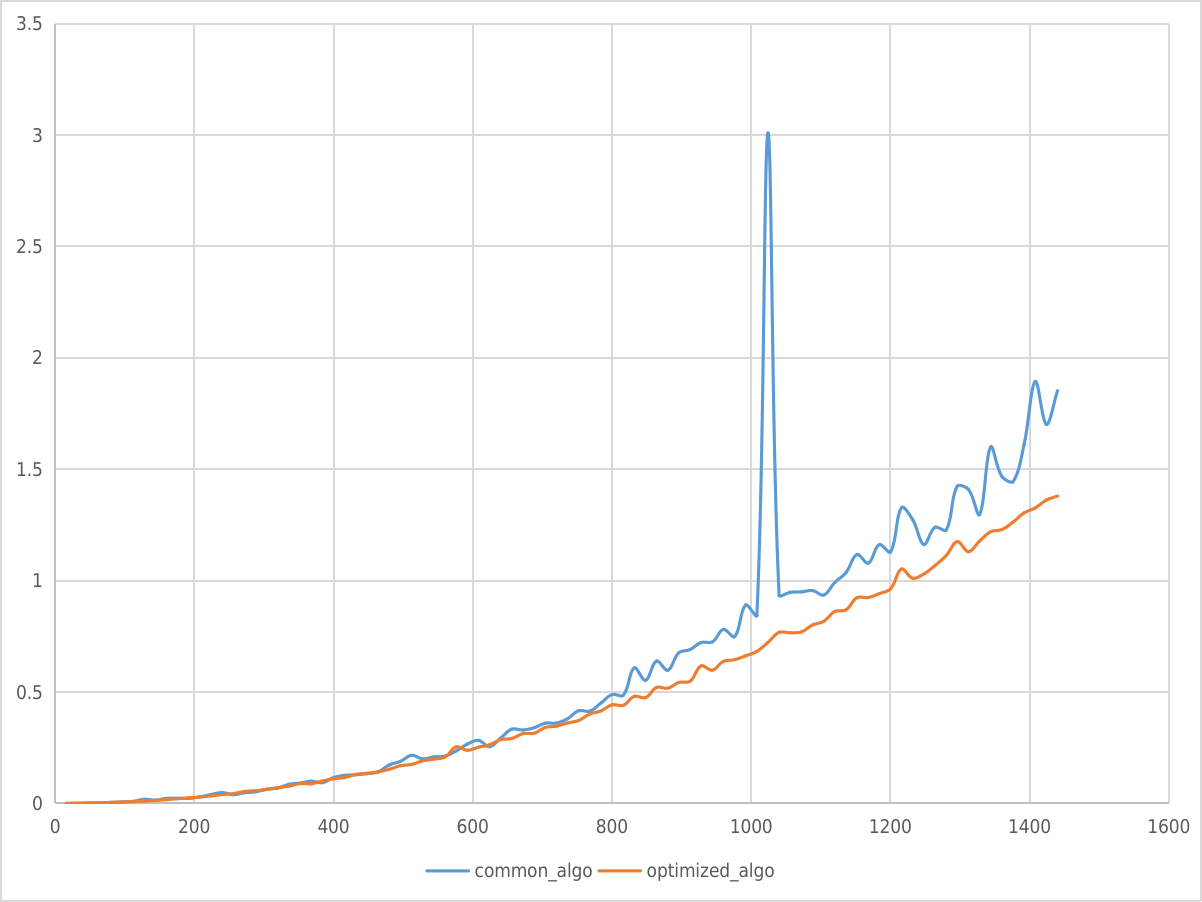
\includegraphics[width=3.2in]{fig/X86_mat_timing.png}
\end{minipage}%
}
\centering
\caption{矩阵列向量点积(矩阵行/列数-运行时间)(单位/秒)}
\label{fig:mat_timing}
\end{figure}

累加实验运行计时的结果如下图所示
\begin{figure}[!htbp]
\centering
\subfigure[ARM平台]{
\begin{minipage}[t]{0.5\linewidth}
\centering
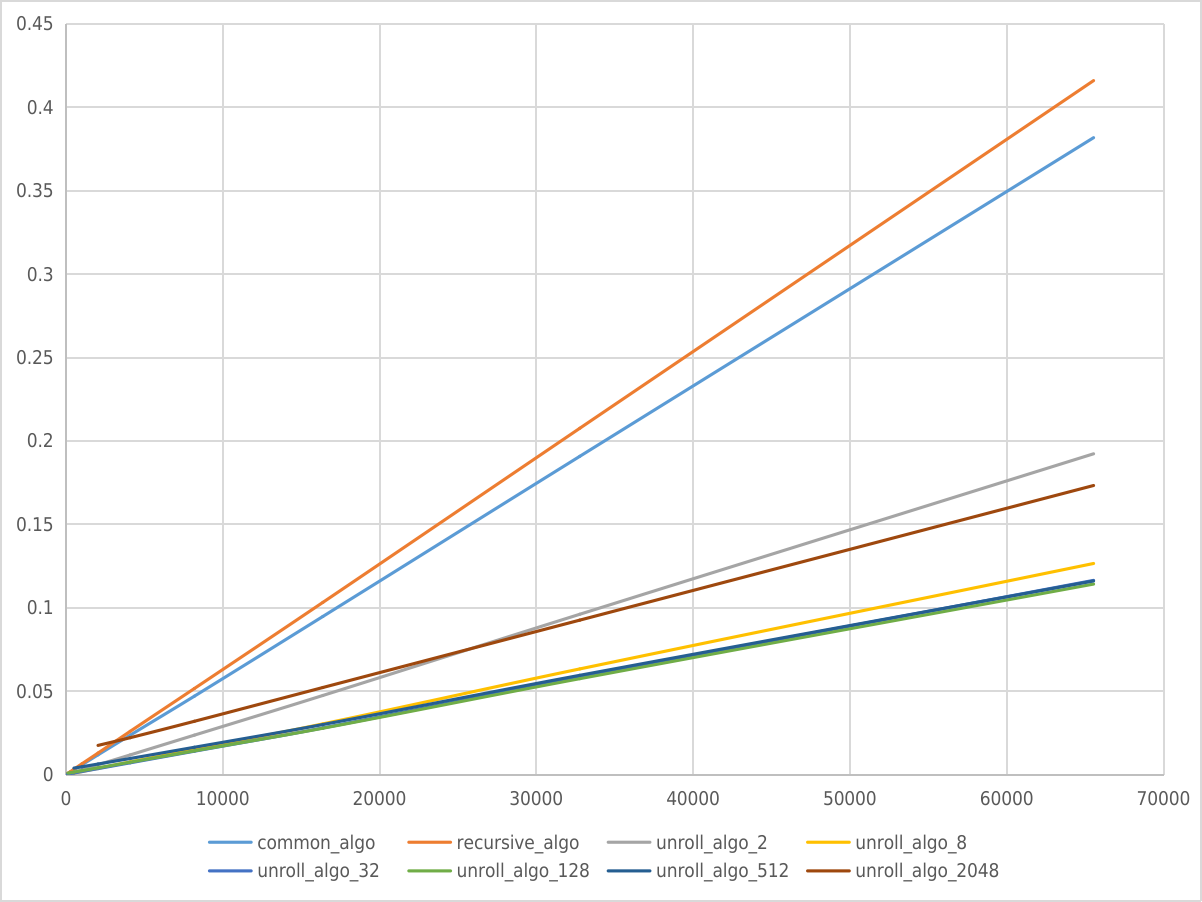
\includegraphics[width=3.2in]{fig/ARM_sum_timing.png}
\label{fig:diff1}
\end{minipage}%
}%
\subfigure[X86平台]{
\begin{minipage}[t]{0.5\linewidth}
\centering
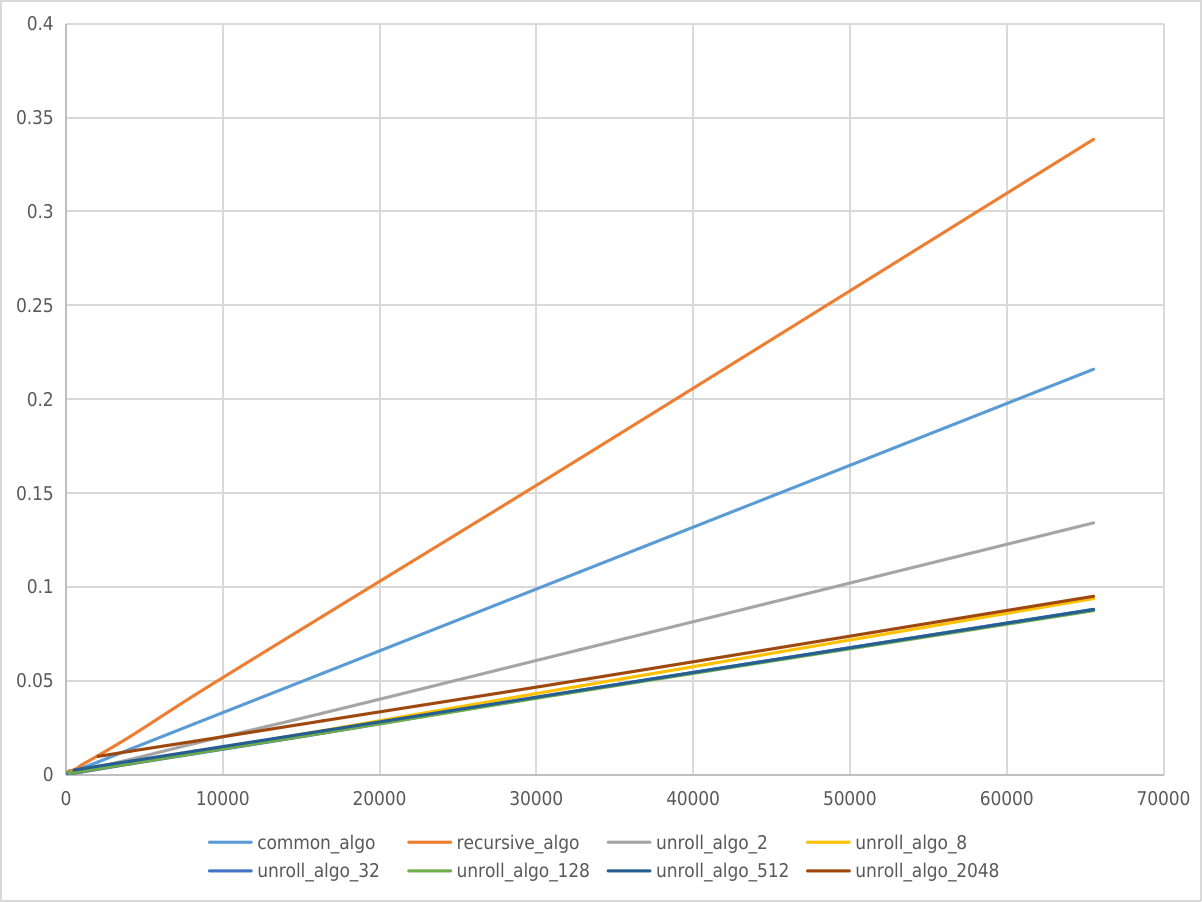
\includegraphics[width=3.2in]{fig/X86_sum_timing.png}
\end{minipage}%
}
\centering
\caption{累加(输入数组长度-运行时间)(单位/秒)}
\label{fig:sum_timing}
\end{figure}


\newpage

\subsection{事件计数}

\begin{table}[!htbp]
\centering
\begin{tabular}{@{}lllll@{}}
\toprule
函数              & \begin{tabular}[c]{@{}l@{}}L1-dcache-\\ load-misses\end{tabular} & L1-dcache-loads & \begin{tabular}[c]{@{}l@{}}L1-dcache-\\ store-misses\end{tabular} & L1-dcache-stores \\ \midrule
common\_algo    & 86.84\%               & 50.00\%         & 86.83\%                & 50.00\%          \\
optimized\_algo & 13.13\%               & 49.99\%         & 13.12\%                & 49.99\%          \\
事件总数            & 30070924              & 3570518704      & 30070932               & 3570537681       \\ \bottomrule
\end{tabular}
\caption{ARM平台下矩阵列向量与向量点积的perf事件计数结果}
\label{table:t_ARM_cache}
\end{table}

\begin{table}[!htbp]
\centering
\begin{tabular}{@{}llll@{}}
\toprule
函数              & L1-dcache-load-misses & L1-dcache-loads & L1-dcache-prefetches \\ \midrule
common\_algo    & 93.55\%               & 50.61\%         & 92.10\%              \\
optimized\_algo & 6.33\%                & 49.23\%         & 7.67\%               \\
事件总数            & 105630435             & 3161589638      & 80585651             \\ \bottomrule
\end{tabular}
\caption{X86平台下矩阵列向量与向量点积的perf事件计数结果}
\label{table:t_x86_cache}
\end{table}

\begin{table}[!htbp]
\centering
\begin{tabular}{@{}llllll@{}}
\toprule
\begin{tabular}[c]{@{}l@{}}优化方法或\\ 循环展开的层数\end{tabular} & cycles       & instructions & CPI    & \begin{tabular}[c]{@{}l@{}}L1-dcache-\\ load-misses\end{tabular} & \begin{tabular}[c]{@{}l@{}}L1-icache-\\ load-misses\end{tabular} \\ \midrule
不优化                                                     & 13.41\%      & 9.19\%       & 0.6296 & 8.24\%                                                           & 0.00\%                                                           \\
递归                                                      & 15.55\%      & 18.67\%      & 0.3594 & 15.01\%                                                          & 0.00\%                                                           \\
2                                                       & 6.73\%       & 7.07\%       & 0.4107 & 6.50\%                                                           & 0.00\%                                                           \\ 
32                                                      & 4.14\%       & 5.21\%       & 0.3429 & 5.06\%                                                           & 0.00\%                                                           \\
512                                                     & 4.15\%       & 5.10\%       & 0.3511 & 6.01\%                                                           & 0.00\%                                                           \\
8192                                                    & 9.89\%       & 6.51\%       & 0.6555 & 8.04\%                                                           & 45.59\%                                                          \\
事件总数                                                    & 122855688833 & 284706374706 & 0.4315 & 633713953                                                        & 2540277364                                                       \\ \bottomrule
\end{tabular}
\caption{ARM平台下累加优化算法的perf事件计数结果}
\label{table:perf_arm_sum}
\end{table}

\begin{table}[!htbp]
\centering
\begin{tabular}{@{}llllll@{}}
\toprule
\begin{tabular}[c]{@{}l@{}}优化方法或\\ 循环展开的层数\end{tabular} & cycles      & instructions & CPI    & \begin{tabular}[c]{@{}l@{}}L1-dcache-\\ load-misses\end{tabular} & \begin{tabular}[c]{@{}l@{}}L1-icache-\\ load-misses\end{tabular} \\ \midrule
不优化                           & 11.81\%     & 6.92\%       & 0.6762 & 5.70\%                                                           & 2.10\%                                                           \\
递归                            & 22.60\%     & 17.53\%      & 0.5108 & 16.13\%                                                          & 4.13\%                                                           \\
2                             & 7.24\%      & 6.70\%       & 0.4281 & 5.51\%                                                           & 1.46\%                                                           \\
32                            & 4.84\%      & 5.76\%       & 0.3329 & 5.36\%                                                           & 1.30\%                                                           \\
512                           & 4.64\%      & 5.59\%       & 0.3288 & 5.38\%                                                           & 2.10\%                                                           \\
8192                          & 5.05\%      & 5.69\%       & 0.3516 & 10.48\%                                                          & 61.37\%                                                          \\
事件总数                          & 52560137817 & 132651641398 & 0.3962 & 889797839                                                        & 60817536                                                                 \\ \bottomrule
\end{tabular}
\caption{X86平台下累加优化算法的perf事件计数结果}
\label{table:perf_X86_sum}
\end{table}



\section{数据分析}

\subsection{Cache优化}
从运行计时的结果图\ref{fig:mat_timing}可以看出,当输入数据规模超出某一个值后,优化的行主访问模式相较于列主访问,在运算时间上产生了较大的优势。根据事件计数的结果表\ref{table:t_ARM_cache},ARM平台上,在L1-dcache-loads、L1-dcache-stores事件数量相差无几的前提下,列主访问的平凡算法所产生的L1-dcache-load-misses、L1-dcache-store-misses的事件数量是行主访问的优化算法的6倍以上。这表明了,列主访问不能最大化发挥cache的潜能,这应该也是行主访问在运行计时上优于列主访问的原因。

\subsection{超标量优化}
从运行计时的结果图\ref{fig:sum_timing}可以看出,无论是两路链式,还是循环展开,其运行速度都优于平凡算法,根据表\ref{table:perf_arm_sum}可以看出,平凡算法的CPI为0.6296,两路链式的CPI为0.4107,而32路链式的CPI为0.3429,这表明在一定范围内,通过增加单次循环中所执行的操作数来进行循环展开的优化,是可以充分利用CPU流水线的设计,得到一定的性能收益的

\subsection{其它问题分析}
\subsubsection{列向量点积数据中的尖峰}
不难注意到,在图\ref{fig:mat_timing}中,ARM平台平凡算法的数据有四个明显的尖峰,除了这四个尖峰外,整个曲线表现出有规律的上下波动。经过几次重复实验后,发现曲线上相近的位置上依然存在着尖峰。并且查看尖峰对应的输入矩阵行数,发现它们恰巧对应着1024、1152、1280、1408(delta=128)这四个数值。

在ARM平台上perf事件计数测量时发现,当矩阵行数为1024时,L1-dcache-load-misses的事件数量比矩阵行数为1025时多了60\%。进一步分析汇编代码,发现这些事件基本都集中在提取矩阵mat[j][i]这个操作上。查阅资料后发现,这个问题可能和cache的结构有关,在鲲鹏920处理器上,Cache划分成了128字节的小块,这种小块被称为Cache Line,而同一个Cache Line是不可被同时访问的。由于出现尖峰的曲线对应的是列主访问的算法,行列数为整倍数的矩阵导致每次从Cache中提取元素都需要跨行访问,导致了额外的开销。也有可能由于超标量的特性,可能存在两条指令同时需要修改同一个Cache Line中的内容的情况,这就造成了伪共享(false sharing)现象,从而导致Cache命中率降低。

\begin{figure}[!htbp]
    \centering
    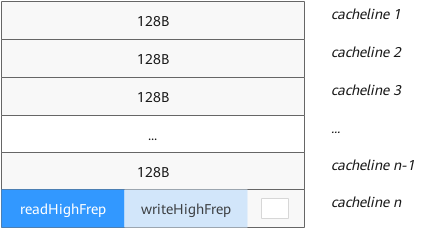
\includegraphics[width=3in]{fig/cache_line.png}
    \caption{Cache的结构 - Cache Line\cite{cacheline}}
    \label{fig:cache_line}
\end{figure}

而在X86平台上,平凡算法的曲线上也存在一个尖峰。perf分析发现,矩阵行数为1024时,branch-misses事件数量比比矩阵行数为1025时多了50\%,而L1-dcache-load-misses的事件数量则是相近的。这可能是由于不同平台的PMU(性能测量单元)或者Cache结构存在着差别,而X86平台上出现尖峰的原因与ARM平台是类似的。也可能是4M的L3 Cache被矩阵占满后,数据存储导致了额外的开销。

其实,在程序性能优化中,Cache Line对齐是非常重要的一环,通过对数据结构的优化,程序可以获得可观的性能提升。

\subsubsection{ARM和X86平台的区别}
不难注意到,在矩阵列向量点积的实验中,ARM平台的总体Cache命中率要比X86平台高很多(99.158\% vs 96.659\%),这可能是由于ARM平台有着更加智能的Cache访问模式,也可能仅仅是因为ARM平台的L1缓存更大(64KB vs 32KB)。此外,不难发现ARM平台的累加的实验的运行时间要比X86平台长得多,这很有可能是因为指令集架构的不同导致的。

\subsubsection{循环展开的层数}
在图\ref{fig:sum_timing}中,可以发现并不是循环展开的路数越多,算法的性能就越好。比如在ARM平台上,2路展开就和8192路展开运行的速度差不多。根据表\ref{table:perf_arm_sum}和表\ref{table:perf_X86_sum}的perf性能分析发现,8192路展开产生了大量的L1-dcache-load-misses和L1-icache-load-misses事件,导致了性能的降低。

导致这现象一方面的原因是,展开循环后的每一行代码依然会产生一定的misses事件,积少成多便降低了Cache命中率。此外,输入数据达到一定规模后,L1 Cache便不再能存下所有的数据了,因此后面的展开会造成大量的性能开销。

这个现象告诉程序设计者们,进行循环展开时的层数也不是越高越好的:展开的层数太高不仅会导致程序体积的变大,还不能给性能带来任何正面的提升。

\subsubsection{递归算法的负优化}
在图\ref{fig:sum_timing}中,显而易见的,递归算法是所有算法中效率最低的一个,这明显是不符合直觉的。分析表\ref{table:perf_arm_sum}和表\ref{table:perf_X86_sum}后发现,递归算法产生了大量的L1-dcache-load-misses事件,这很有可能是因为递归算法需要进行大量不连续内存的访问,跨越Cache Line或者Cache Line伪共享很可能是命中率降低的罪魁祸首。

此外,递归算法的代码本身就比平凡算法和多路链式算法要复杂,多出来的变量也很可能造成了不小的额外开销。

\newpage
\bibliographystyle{plain}
\bibliography{reference.bib} 

\end{document}